\documentclass[12pt]{article}
\usepackage[cm]{fullpage}
\usepackage{fancyhdr}
\pagestyle{fancy}
\fancyhf{}
\cfoot{2016}
\renewcommand{\headrulewidth}{0pt}

\usepackage{pdfpages}

\begin{document}
\begin{center}
{\Huge Unorchestrated Structure for Strings with Soloist}
\end{center}

\vspace{0.2cm}

\begin{flushright}
Adam Tindale
\end{flushright}

\vspace{0.3cm}

\hrule

\vspace{0.1cm}

\textcircled{\raisebox{-0.9pt}{1}}

\begin{tabular}{l l}
\begin{minipage}{0.5\textwidth}
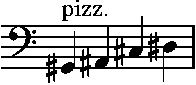
\includegraphics[scale=1.5]{gacdbasspizz.pdf}
\end{minipage}
&
\begin{minipage}{0.5\textwidth}
Play notes in any octave with any rhythm.
\end{minipage}
\end{tabular}

\vspace{0.3cm}

\hrule

\vspace{0.1cm}

\textcircled{\raisebox{-0.9pt}{2}}


\begin{tabular}{l l}
\begin{minipage}{0.5\textwidth}
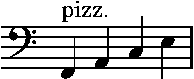
\includegraphics[scale=1.5]{facebasspizz.pdf} 
\end{minipage}
&
\begin{minipage}{0.5\textwidth}
Play notes in any octave with any rhythm.
\end{minipage}
\end{tabular}

\vspace{0.3cm}

\hrule

\vspace{0.1cm}

\textcircled{\raisebox{-0.9pt}{3}}



\begin{tabular}{l l}
\begin{minipage}{0.5\textwidth}
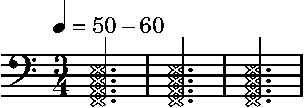
\includegraphics[scale=1.5]{melodybass.pdf}
\end{minipage}
&
\begin{minipage}{0.4\textwidth}
Pick any of the notes for each of the three bars. Play each phrase with different notes in different orders. You may rest for any number of bars between phrases.
\end{minipage}
\end{tabular}
\vspace{0.3cm}

\hrule

\vspace{0.1cm}

\textcircled{\raisebox{-0.9pt}{4}}

\begin{tabular}{l l}
\begin{minipage}{0.5\textwidth}
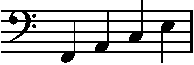
\includegraphics[scale=1.5]{facebass.pdf}
\end{minipage}
&
\begin{minipage}{0.4\textwidth}
Play notes in any octave with any rhythm. Imitate soloist if you choose. 
\end{minipage}
\end{tabular}

\vspace{0.3cm}

\hrule

\vspace{0.1cm}

\textcircled{\raisebox{-0.9pt}{5}}

\begin{tabular}{l l}
\begin{minipage}{0.5\textwidth}
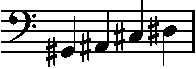
\includegraphics[scale=1.5]{gacdbass.pdf}
\end{minipage}
&
\begin{minipage}{0.4\textwidth}
Play notes in any octave with any rhythm. Imitate soloist if you choose. 
\end{minipage}
\end{tabular}

\vspace{0.3cm}

\hrule

\end{document}
